%The MERLIN dataset was first phase-shifted to NGC~5195, and then corrected for primary beam effects using PBCOR\footnote{Here the standard VLA airy disk primary beam is used. An accurate primary beam model is provided for MERLIN/e-MERLIN that takes into account the 76-m Lovell and the 32-m Cambridge dishes. However, this up-weights all baselines to Lovell and Cambridge, increasing the baseline making the detection of the low surface brightness emission difficult.}, exported and finally imaged in CASA. The final naturally weighted contour map is also included in \fig~\ref{fig:MERLINimg}. 
%combined all three datasets and found no emission above 5*36.8 \mujybm near the bubbles.


%\subsection{Flux Measurements}


% \subsection{Archival VLA - Polarisation}

% \textbf{NGC~5195 has been the focus of many polarisation studies with the VLA. \cite{Horellouetal92} observed NGC~5195 for 12 hours at 18 and 20~cm simultaneously with the VLA in the most compact configuration (D-array). Their pre-calibrated 20~cm linear polarisation intensity (PI) map is available online from the \textit{Atlas of Galaxies}\footnote{\url{http://www.mpifr-bonn.mpg.de/atlasmag}}. \Fig~\ref{fig:pol} displays the 20~cm PI gray-scale map for NGC~5195. In addition, \cite{Fletcheretal2011} observed NGC~5195 with the VLA in C configuration at 6 cm in full polarisation. Their final Q and U stokes images were obtained from A. Fletcher (private communication)}. 

% \textbf{The polarisation angle vectors were obtained from the Q and U stokes images using the AIPS task COMB. The magnetic field vectors (which is the polarisation angle vectors rotated by 90\deg) is displayed in  \fig~\ref{fig:pol} with the VLA 1.4~GHz contours from \fig~\ref{fig:VLAMaps} over plotted.} 
 

% %-------------------------------------------
% \begin{figure}
% {\centering
% 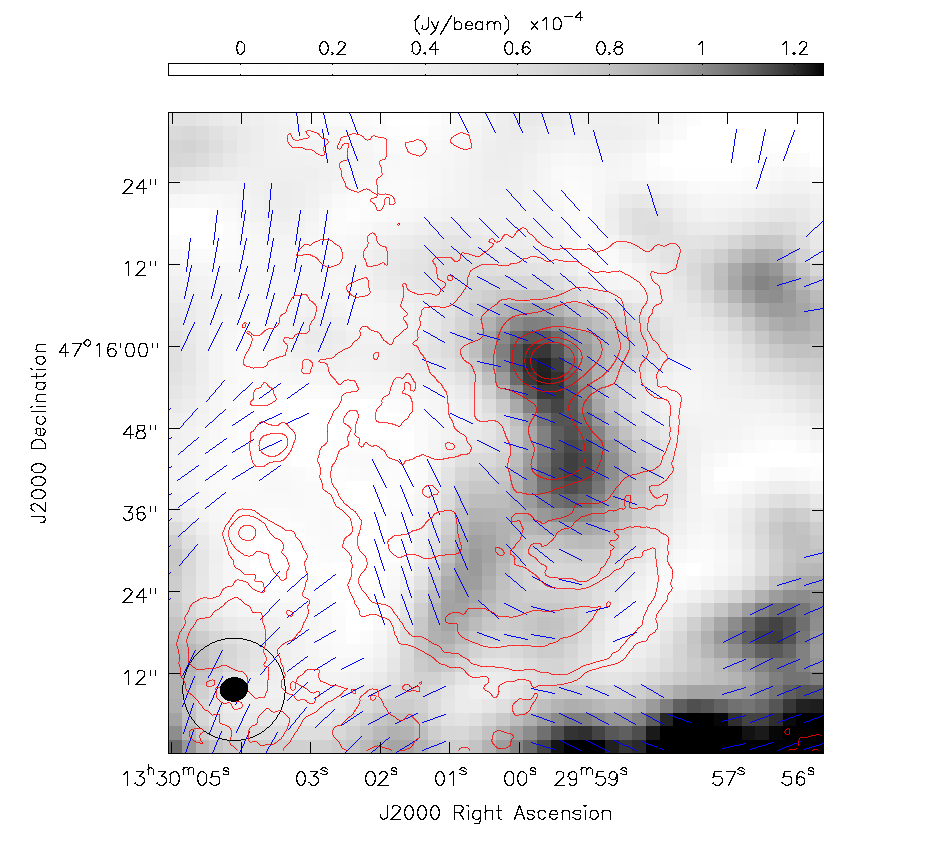
\includegraphics[scale=0.35]{M51b_20PI_6PA_20cont.png}
% \smallskip
% \caption{Image showing the VLA 20~cm PI (gray-scale) map \citep{Horellouetal92}, with the 6~cm magnetic-field vectors of polarised emission (blue) \citep{Fletcheretal2011} and the VLA 1.4~GHz total intensity contour map from this paper (contours are the same as \fig~\ref{fig:VLAMaps}a. The rms noise of the PI map is 35 \mujybm.}
% \label{fig:pol}
% }
% \end{figure}
% %------------------------------------------



% \subsection{Radio polarisation and magnetic fields}

% \textbf{Linear polarisation is an important diagnostic of non-thermal radio emission \citep{BFM2002} since synchrotron emission is inherently polarised (see CITE DAVID BOOK). In AGNs and galaxies it has been used to demonstrate that magnetic fields are present, and that shocks propagate in jets, compressing the magnetic fields (e.g. \citealt{Laing80,BFM2002,Wardle2013,Mulcahyetal2014}).}
 
% \Fig~\ref{fig:pol} shows the linear polarisation intensity at 20~cm and the magnetic field vectors, along with the VLA 1.4 GHz contours (from \fig~\ref{fig:VLAMaps}). The image shows PI above 105 \mujybm (3$\sigma$) along the jet, while the PI in the arc is $\<$~105 \mujybm.

% The magnetic field vectors along the jet are at $\sim$45\deg to the \textbf{direction of the jet}, while it appears to trace the arc. Magnetic fields are known to be transverse to the direction of the shock (e.g. jets \citealt{Laing80,Wardle2013}), resulting from the compression of a completely disordered magnetic field by the shock-wave \citep{Laing80}. However, it is possible for the magnetic field to be partially aligned \citep{Wardle2013}. This can occur when the shock from the jet is bent by an external pressure or density gradient forming an oblique shock that can misalign the polarization angle, and hence the magnetic field angle \citep{Hughes2005,Hughesetal2011}. The radio-arc and jet are located in a region of higher density, due to the interaction of NGC~5195 with NGC~5194, that may have resulted in the observed magnetic field.

% While there is possible contamination of the polarisation and hence magnetic field due to NGC~5194, the alignment with the radio-arc and jet strongly suggests that the magnetic field and polarisation in \fig~\ref{fig:pol} are from NGC~5195. Time have been awarded on the Karl G. Jansky VLA (JVLA) for more sensitive polarised observations centred on NGC~5195, the results will be presented in a later publication.






% %\subsection{in-Active Galactic Nuclei?}
% \section{An in-Active Galactic Nucleus?}


% The $\sim$150-50\,mas resolution e-MERLIN observations show the existence of a parsec-scale core-jet source, typical of LLAGNS, within the nucleus of NGC~5195. However, a recent high-resolution survey of the M51 system with the European 
% VLBI Network (EVN) at 18~cm failed to detect any emission arising from the NGC~5195 core above a limit of 132~\mujybm~ \citep{Rampadarathetal15}. This places an upper limit on the power output of the AGN core of $\approx\,10^{18}\,{\rm W\,Hz^{-1}}$ ($10^{34}\,{\rm erg\,s^{-1}}$) and the brightness temperature ${\rm T_{B}}\leq\,9\,\times\,10^{5}$. Since the peak flux density of the partially-resolved e-MERLIN L-band source ($\approx 400$~\mujybm) is well above the EVN detection limit (132~\mujybm), one would expect the AGN core to be visible in the EVN map. 
% The lack of a compact VLBI core, representing the base of the jet, suggests either it is currently in a state of inactivity or resolved out at lower frequencies.

% Jet quenching is commonly observed in stellar-mass BH X-ray binaries, when they switch from the hard state (associated with a steady jet) to the high/soft state \citep{Fender+2004}, at an Eddington ratio of a few 10$^{-2}$. The transition is caused by the collapse of the hot accretion flow into a geometrically thin, radiatively efficient accretion disk. A similar mechanism may operate in AGN at comparable Eddington ratios \citep{Kordingetal2006c}. However, this is clearly not the case in NGC 5195, as we have shown that its Eddington ratio is a few 10$^{-6}$, safely in the low/hard state. One possibility is that the accretion power of the SMBH, and therefore also the radio emission from the base of the compact jet, varies by a factor $>$3 over a timescale of several years, explaining the discrepancy between EVN (2011) and both MERLIN (2005) and e-MERLIN (2015) observations. Radio and X-ray variability over a few weeks to years' time-scales is well documented in other low-luminosity nearby AGN \citep{Markoffetal2008,Pian2010,Kingetal2016}. 


% %Another possibility is that we have over-estimated the current X-ray luminosity of the nuclear SMBH, and therefore also the expected radio luminosity of its compact jet (via the fundamental plane relation, see \sect~\ref{sec:xrays_orign}). This may be the case if some of the hard X-ray emission detected by {\it Chandra} comes not from the compact nuclear source but from stellar-mass X-ray binaries or hot gas in the nuclear region, perhaps the same gas that is causing the marginally resolved radio emission. We leave a spectral and time-variability study of the nuclear X-ray source to follow-up work.
% Another possibility is that the nuclear radio emission at lower frequencies is absorbed by an optically thick screen of ionised gas. Evidence for this comes from the downturn observed in the radio spectra of compact radio sources for example, supernova remnants \citep{Tingay2004,LT06} and AGNs \citep{Bicknelletal1997, Pedlaretal1998,Kamenoetal2003}. Indeed, the X-ray spectrum shows evidence for an additional thermal-plasma component (see \sect~\ref{sec:xrays_orign}), which may be evidence of hot ionised gas surrounding the nucleus. 
